\documentclass[11pt,fleqn, oneside,openany]{extbook} % Default font size and left-justified equations

% use this list: https://www.educative.io/blog/google-coding-interview

%%%%%%%%%%%%%%%%%%%%%%%%%%%%%%%%%%%%%%%%%%%%
%               Structure
%%%%%%%%%%%%%%%%%%%%%%%%%%%%%%%%%%%%%%%%%%%%
%%%%%%%%%%%%%%%%%%%%%%%%%%%%%%%%%%%%%%%%%
% The Legrand Orange Book
% Structural Definitions File
% Version 2.0 (9/2/15)
%
% Original author:
% Mathias Legrand (legrand.mathias@gmail.com) with modifications by:
% Vel (vel@latextemplates.com)
% 
% This file has been downloaded from:
% http://www.LaTeXTemplates.com
%
% License:
% CC BY-NC-SA 3.0 (http://creativecommons.org/licenses/by-nc-sa/3.0/)
%
%%%%%%%%%%%%%%%%%%%%%%%%%%%%%%%%%%%%%%%%%

%----------------------------------------------------------------------------------------
%	VARIOUS REQUIRED PACKAGES AND CONFIGURATIONS
%----------------------------------------------------------------------------------------

\usepackage[top=3cm,bottom=3cm,left=3cm,right=3cm,headsep=10pt,a4paper]{geometry} % Page margins

\usepackage{graphicx} % Required for including pictures
\graphicspath{{images/}} % Specifies the directory where pictures are stored

\usepackage{lipsum} % Inserts dummy text

\usepackage{tikz} % Required for drawing custom shapes

\usepackage[english]{babel} % English language/hyphenation

\usepackage{enumitem} % Customize lists
\setlist{nolistsep} % Reduce spacing between bullet points and numbered lists

\usepackage{booktabs} % Required for nicer horizontal rules in tables

\usepackage{xcolor} % Required for specifying colors by name
\definecolor{ocre}{RGB}{243,102,25} % Define the orange color used for highlighting throughout the book

%----------------------------------------------------------------------------------------
%	FONTS
%----------------------------------------------------------------------------------------

\usepackage{avant} % Use the Avantgarde font for headings
%\usepackage{times} % Use the Times font for headings
\usepackage{mathptmx} % Use the Adobe Times Roman as the default text font together with math symbols from the Sym­bol, Chancery and Com­puter Modern fonts

\usepackage{microtype} % Slightly tweak font spacing for aesthetics
\usepackage[utf8]{inputenc} % Required for including letters with accents
\usepackage[T1]{fontenc} % Use 8-bit encoding that has 256 glyphs

%----------------------------------------------------------------------------------------
%	BIBLIOGRAPHY AND INDEX
%----------------------------------------------------------------------------------------

\usepackage[citestyle=numeric,sorting=nyt,sortcites=true,autopunct=true,babel=hyphen,hyperref=true,abbreviate=false,backref=true,backend=biber]{biblatex}
\addbibresource{sources/bibliography.bib}
\defbibheading{bibempty}{}

\usepackage{calc} % For simpler calculation - used for spacing the index letter headings correctly
\usepackage{makeidx} % Required to make an index
\makeindex % Tells LaTeX to create the files required for indexing

%----------------------------------------------------------------------------------------
%	MAIN TABLE OF CONTENTS
%----------------------------------------------------------------------------------------

\usepackage{titletoc} % Required for manipulating the table of contents

\contentsmargin{0cm} % Removes the default margin

% Part text styling
\titlecontents{part}[0cm]
{\addvspace{20pt}\centering\large\bfseries}
{}
{}
{}

% Chapter text styling
\titlecontents{chapter}[1.25cm] % Indentation
{\addvspace{12pt}\large\sffamily\bfseries} % Spacing and font options for chapters
{\color{ocre!60}\contentslabel[\Large\thecontentslabel]{1.25cm}\color{ocre}} % Chapter number
{\color{ocre}}  
{\color{ocre!60}\normalsize\;\titlerule*[.5pc]{.}\;\thecontentspage} % Page number

% Section text styling
\titlecontents{section}[1.25cm] % Indentation
{\addvspace{3pt}\sffamily\bfseries} % Spacing and font options for sections
{\contentslabel[\thecontentslabel]{1.25cm}} % Section number
{}
{\hfill\color{black}\thecontentspage} % Page number
[]

% Subsection text styling
\titlecontents{subsection}[1.25cm] % Indentation
{\addvspace{1pt}\sffamily\small} % Spacing and font options for subsections
{\contentslabel[\thecontentslabel]{1.25cm}} % Subsection number
{}
{\ \titlerule*[.5pc]{.}\;\thecontentspage} % Page number
[]

% List of figures
\titlecontents{figure}[0em]
{\addvspace{-5pt}\sffamily}
{\thecontentslabel\hspace*{1em}}
{}
{\ \titlerule*[.5pc]{.}\;\thecontentspage}
[]

% List of tables
\titlecontents{table}[0em]
{\addvspace{-5pt}\sffamily}
{\thecontentslabel\hspace*{1em}}
{}
{\ \titlerule*[.5pc]{.}\;\thecontentspage}
[]

%----------------------------------------------------------------------------------------
%	MINI TABLE OF CONTENTS IN PART HEADS
%----------------------------------------------------------------------------------------

% Chapter text styling
\titlecontents{lchapter}[0em] % Indenting
{\addvspace{15pt}\large\sffamily\bfseries} % Spacing and font options for chapters
{\color{ocre}\contentslabel[\Large\thecontentslabel]{1.25cm}\color{ocre}} % Chapter number
{}  
{\color{ocre}\normalsize\sffamily\bfseries\;\titlerule*[.5pc]{.}\;\thecontentspage} % Page number

% Section text styling
\titlecontents{lsection}[0em] % Indenting
{\sffamily\small} % Spacing and font options for sections
{\contentslabel[\thecontentslabel]{1.25cm}} % Section number
{}
{}

% Subsection text styling
\titlecontents{lsubsection}[.5em] % Indentation
{\normalfont\footnotesize\sffamily} % Font settings
{}
{}
{}

%----------------------------------------------------------------------------------------
%	PAGE HEADERS
%----------------------------------------------------------------------------------------

\usepackage{fancyhdr} % Required for header and footer configuration

\pagestyle{fancy}
\renewcommand{\chaptermark}[1]{\markboth{\sffamily\normalsize\bfseries\chaptername\ \thechapter.\ #1}{}} % Chapter text font settings
\renewcommand{\sectionmark}[1]{\markright{\sffamily\normalsize\thesection\hspace{5pt}#1}{}} % Section text font settings
\fancyhf{} \fancyhead[LE,RO]{\sffamily\normalsize\thepage} % Font setting for the page number in the header
\fancyhead[LO]{\rightmark} % Print the nearest section name on the left side of odd pages
\fancyhead[RE]{\leftmark} % Print the current chapter name on the right side of even pages
\renewcommand{\headrulewidth}{0.5pt} % Width of the rule under the header
\addtolength{\headheight}{2.5pt} % Increase the spacing around the header slightly
\renewcommand{\footrulewidth}{0pt} % Removes the rule in the footer
\fancypagestyle{plain}{\fancyhead{}\renewcommand{\headrulewidth}{0pt}} % Style for when a plain pagestyle is specified

% Removes the header from odd empty pages at the end of chapters
\makeatletter
\renewcommand{\cleardoublepage}{
\clearpage\ifodd\c@page\else
\hbox{}
\vspace*{\fill}
\thispagestyle{empty}
\newpage
\fi}

%----------------------------------------------------------------------------------------
%	THEOREM STYLES
%----------------------------------------------------------------------------------------


\usepackage{amsmath,amsfonts,amssymb,amsthm,mathtools} % For math equations, theorems, symbols, etc
\DeclarePairedDelimiter\ceil{\lceil}{\rceil}
\DeclarePairedDelimiter\floor{\lfloor}{\rfloor}

\newcommand{\intoo}[2]{\mathopen{]}#1\,;#2\mathclose{[}}
\newcommand{\ud}{\mathop{\mathrm{{}d}}\mathopen{}}
\newcommand{\intff}[2]{\mathopen{[}#1\,;#2\mathclose{]}}
\newtheorem{notation}{Notation}[chapter]

% Boxed/framed environments
\newtheoremstyle{ocrenumbox}% % Theorem style name
{0pt}% Space above
{0pt}% Space below
{\normalfont}% % Body font
{}% Indent amount
{\small\bf\sffamily\color{ocre}}% % Theorem head font
{\;}% Punctuation after theorem head
{0.25em}% Space after theorem head
{\small\sffamily\color{ocre}\thmname{#1}\nobreakspace\thmnumber{\@ifnotempty{#1}{}\@upn{#2}}% Theorem text (e.g. Theorem 2.1)
\thmnote{\nobreakspace\the\thm@notefont\sffamily\bfseries\color{black}---\nobreakspace#3.}} % Optional theorem note
\renewcommand{\qedsymbol}{$\blacksquare$}% Optional qed square

\newtheoremstyle{blacknumex}% Theorem style name
{5pt}% Space above
{5pt}% Space below
{\normalfont}% Body font
{} % Indent amount
{\small\bf\sffamily}% Theorem head font
{\;}% Punctuation after theorem head
{0.25em}% Space after theorem head
{\small\sffamily{\tiny\ensuremath{\blacksquare}}\nobreakspace\thmname{#1}\nobreakspace\thmnumber{\@ifnotempty{#1}{}\@upn{#2}}% Theorem text (e.g. Theorem 2.1)
\thmnote{\nobreakspace\the\thm@notefont\sffamily\bfseries---\nobreakspace#3.}}% Optional theorem note

\newtheoremstyle{blacknumbox} % Theorem style name
{0pt}% Space above
{0pt}% Space below
{\normalfont}% Body font
{}% Indent amount
{\small\bf\sffamily}% Theorem head font
{\;}% Punctuation after theorem head
{0.25em}% Space after theorem head
{\small\sffamily\thmname{#1}\nobreakspace\thmnumber{\@ifnotempty{#1}{}\@upn{#2}}% Theorem text (e.g. Theorem 2.1)
\thmnote{\nobreakspace\the\thm@notefont\sffamily\bfseries---\nobreakspace#3.}}% Optional theorem note

% Non-boxed/non-framed environments
\newtheoremstyle{ocrenum}% % Theorem style name
{5pt}% Space above
{5pt}% Space below
{\normalfont}% % Body font
{}% Indent amount
{\small\bf\sffamily\color{ocre}}% % Theorem head font
{\;}% Punctuation after theorem head
{0.25em}% Space after theorem head
{\small\sffamily\color{ocre}\thmname{#1}\nobreakspace\thmnumber{\@ifnotempty{#1}{}\@upn{#2}}% Theorem text (e.g. Theorem 2.1)
\thmnote{\nobreakspace\the\thm@notefont\sffamily\bfseries\color{black}---\nobreakspace#3.}} % Optional theorem note
\renewcommand{\qedsymbol}{$\blacksquare$}% Optional qed square
\makeatother

% Defines the theorem text style for each type of theorem to one of the three styles above
\newcounter{dummy} 
\numberwithin{dummy}{section}
\theoremstyle{ocrenumbox}
\newtheorem{theoremeT}[dummy]{Theorem}

\newtheorem{problem}{Exercise}[chapter]
\newtheorem{exerciseT}{Problem}
\theoremstyle{blacknumex}
\newtheorem{solution}{Solution}[chapter]
\newtheorem{solutionT}{solution}[chapter]
\theoremstyle{blacknumex}
\newtheorem{exampleT}{Example}[chapter]
\theoremstyle{blacknumbox}
\newtheorem{vocabulary}{Vocabulary}[chapter]
\newtheorem{definitionT}{Definition}[section]
\newtheorem{corollaryT}[dummy]{Corollary}
\theoremstyle{ocrenum}
\newtheorem{proposition}[dummy]{Proposition}

%----------------------------------------------------------------------------------------
%	DEFINITION OF COLORED BOXES
%----------------------------------------------------------------------------------------

\RequirePackage[framemethod=default]{mdframed} % Required for creating the theorem, definition, exercise and corollary boxes

% Theorem box
\newmdenv[skipabove=7pt,
skipbelow=7pt,
backgroundcolor=black!5,
linecolor=ocre,
innerleftmargin=5pt,
innerrightmargin=5pt,
innertopmargin=5pt,
leftmargin=0cm,
rightmargin=0cm,
innerbottommargin=5pt]{tBox}

% Exercise box	  
\newmdenv[skipabove=7pt,
skipbelow=7pt,
rightline=false,
leftline=true,
topline=false,
bottomline=false,
backgroundcolor=ocre!10,
linecolor=ocre,
innerleftmargin=5pt,
innerrightmargin=5pt,
innertopmargin=5pt,
innerbottommargin=5pt,
leftmargin=0cm,
rightmargin=0cm,
linewidth=4pt]{eBox}	

% Definition box
\newmdenv[skipabove=7pt,
skipbelow=7pt,
rightline=false,
leftline=true,
topline=false,
bottomline=false,
linecolor=ocre,
innerleftmargin=5pt,
innerrightmargin=5pt,
innertopmargin=0pt,
leftmargin=0cm,
rightmargin=0cm,
linewidth=4pt,
innerbottommargin=0pt]{dBox}	

% Corollary box
\newmdenv[skipabove=7pt,
skipbelow=7pt,
rightline=false,
leftline=true,
topline=false,
bottomline=false,
linecolor=gray,
backgroundcolor=black!5,
innerleftmargin=5pt,
innerrightmargin=5pt,
innertopmargin=5pt,
leftmargin=0cm,
rightmargin=0cm,
linewidth=4pt,
innerbottommargin=5pt]{cBox}

% Creates an environment for each type of theorem and assigns it a theorem text style from the "Theorem Styles" section above and a colored box from above
\newenvironment{theorem}{\begin{tBox}\begin{theoremeT}}{\end{theoremeT}\end{tBox}}
\newenvironment{exercise}{\begin{eBox}\begin{exerciseT}}{\hfill{\color{ocre}\tiny\ensuremath{\blacksquare}}\end{exerciseT}\end{eBox}}				  
\newenvironment{definition}{\begin{dBox}\begin{definitionT}}{\end{definitionT}\end{dBox}}	
\newenvironment{example}{\begin{exampleT}}{\hfill{\tiny\ensuremath{\blacksquare}}\end{exampleT}}		
\newenvironment{corollary}{\begin{cBox}\begin{corollaryT}}{\end{corollaryT}\end{cBox}}	

%----------------------------------------------------------------------------------------
%	REMARK ENVIRONMENT
%----------------------------------------------------------------------------------------

\newenvironment{remark}{\par\vspace{10pt}\small % Vertical white space above the remark and smaller font size
\begin{list}{}{
\leftmargin=35pt % Indentation on the left
\rightmargin=25pt}\item\ignorespaces % Indentation on the right
\makebox[-2.5pt]{\begin{tikzpicture}[overlay]
\node[draw=ocre!60,line width=1pt,circle,fill=ocre!25,font=\sffamily\bfseries,inner sep=2pt,outer sep=0pt] at (-15pt,0pt){\textcolor{ocre}{R}};\end{tikzpicture}} % Orange R in a circle
\advance\baselineskip -1pt}{\end{list}\vskip5pt} % Tighter line spacing and white space after remark

%----------------------------------------------------------------------------------------
%	SECTION NUMBERING IN THE MARGIN
%----------------------------------------------------------------------------------------

\makeatletter
\renewcommand{\@seccntformat}[1]{\llap{\textcolor{ocre}{\csname the#1\endcsname}\hspace{1em}}}                    
\renewcommand{\section}{\@startsection{section}{1}{\z@}
{-4ex \@plus -1ex \@minus -.4ex}
{1ex \@plus.2ex }
{\normalfont\large\sffamily\bfseries}}
\renewcommand{\subsection}{\@startsection {subsection}{2}{\z@}
{-3ex \@plus -0.1ex \@minus -.4ex}
{0.5ex \@plus.2ex }
{\normalfont\sffamily\bfseries}}
\renewcommand{\subsubsection}{\@startsection {subsubsection}{3}{\z@}
{-2ex \@plus -0.1ex \@minus -.2ex}
{.2ex \@plus.2ex }
{\normalfont\small\sffamily\bfseries}}                        
\renewcommand\paragraph{\@startsection{paragraph}{4}{\z@}
{-2ex \@plus-.2ex \@minus .2ex}
{.1ex}
{\normalfont\small\sffamily\bfseries}}

%----------------------------------------------------------------------------------------
%	PART HEADINGS
%----------------------------------------------------------------------------------------

% numbered part in the table of contents
\newcommand{\@mypartnumtocformat}[2]{%
\setlength\fboxsep{0pt}%
\noindent\colorbox{ocre!20}{\strut\parbox[c][.7cm]{\ecart}{\color{ocre!70}\Large\sffamily\bfseries\centering#1}}\hskip\esp\colorbox{ocre!40}{\strut\parbox[c][.7cm]{\linewidth-\ecart-\esp}{\Large\sffamily\centering#2}}}%
%%%%%%%%%%%%%%%%%%%%%%%%%%%%%%%%%%
% unnumbered part in the table of contents
\newcommand{\@myparttocformat}[1]{%
\setlength\fboxsep{0pt}%
\noindent\colorbox{ocre!40}{\strut\parbox[c][.7cm]{\linewidth}{\Large\sffamily\centering#1}}}%
%%%%%%%%%%%%%%%%%%%%%%%%%%%%%%%%%%
\newlength\esp
\setlength\esp{4pt}
\newlength\ecart
\setlength\ecart{1.2cm-\esp}
\newcommand{\thepartimage}{}%
\newcommand{\partimage}[1]{\renewcommand{\thepartimage}{#1}}%
\def\@part[#1]#2{%
\ifnum \c@secnumdepth >-2\relax%
\refstepcounter{part}%
\addcontentsline{toc}{part}{\texorpdfstring{\protect\@mypartnumtocformat{\thepart}{#1}}{\partname~\thepart\ ---\ #1}}
\else%
\addcontentsline{toc}{part}{\texorpdfstring{\protect\@myparttocformat{#1}}{#1}}%
\fi%
\startcontents%
\markboth{}{}%
{\thispagestyle{empty}%
\begin{tikzpicture}[remember picture,overlay]%
\node at (current page.north west){\begin{tikzpicture}[remember picture,overlay]%	
\fill[ocre!20](0cm,0cm) rectangle (\paperwidth,-\paperheight);
\node[anchor=north] at (4cm,-3.25cm){\color{ocre!40}\fontsize{220}{100}\sffamily\bfseries\@Roman\c@part}; 
\node[anchor=south east] at (\paperwidth-1cm,-\paperheight+1cm){\parbox[t][][t]{8.5cm}{
\printcontents{l}{0}{\setcounter{tocdepth}{1}}%
}};
\node[anchor=north east] at (\paperwidth-1.5cm,-3.25cm){\parbox[t][][t]{15cm}{\strut\raggedleft\color{white}\fontsize{30}{30}\sffamily\bfseries#2}};
\end{tikzpicture}};
\end{tikzpicture}}%
\@endpart}
\def\@spart#1{%
\startcontents%
\phantomsection
{\thispagestyle{empty}%
\begin{tikzpicture}[remember picture,overlay]%
\node at (current page.north west){\begin{tikzpicture}[remember picture,overlay]%	
\fill[ocre!20](0cm,0cm) rectangle (\paperwidth,-\paperheight);
\node[anchor=north east] at (\paperwidth-1.5cm,-3.25cm){\parbox[t][][t]{15cm}{\strut\raggedleft\color{white}\fontsize{30}{30}\sffamily\bfseries#1}};
\end{tikzpicture}};
\end{tikzpicture}}
\addcontentsline{toc}{part}{\texorpdfstring{%
\setlength\fboxsep{0pt}%
\noindent\protect\colorbox{ocre!40}{\strut\protect\parbox[c][.7cm]{\linewidth}{\Large\sffamily\protect\centering #1\quad\mbox{}}}}{#1}}%
\@endpart}
\def\@endpart{\vfil\newpage
\if@twoside
\if@openright
\null
\thispagestyle{empty}%
\newpage
\fi
\fi
\if@tempswa
\twocolumn
\fi}

%----------------------------------------------------------------------------------------
%	CHAPTER HEADINGS
%----------------------------------------------------------------------------------------

% A switch to conditionally include a picture, implemented by  Christian Hupfer
\newif\ifusechapterimage
\usechapterimagetrue
\newcommand{\thechapterimage}{}%
\newcommand{\chapterimage}[1]{\ifusechapterimage\renewcommand{\thechapterimage}{#1}\fi}%
\def\@makechapterhead#1{%
{\parindent \z@ \raggedright \normalfont
\ifnum \c@secnumdepth >\m@ne
\if@mainmatter
\begin{tikzpicture}[remember picture,overlay]
\node at (current page.north west)
{\begin{tikzpicture}[remember picture,overlay]
\node[anchor=north west,inner sep=0pt] at (0,0) {\ifusechapterimage\includegraphics[width=\paperwidth]{\thechapterimage}\fi};
\draw[anchor=west] (\Gm@lmargin,-4cm) node [line width=2pt,rounded corners=15pt,draw=ocre,fill=white,fill opacity=0.5,inner sep=15pt]{\strut\makebox[22cm]{}};
\draw[anchor=west] (\Gm@lmargin+.3cm,-4cm) node {\huge\sffamily\bfseries\color{black}\thechapter. #1\strut};
\end{tikzpicture}};
\end{tikzpicture}
\else
\begin{tikzpicture}[remember picture,overlay]
\node at (current page.north west)
{\begin{tikzpicture}[remember picture,overlay]
\node[anchor=north west,inner sep=0pt] at (0,0) {\ifusechapterimage\includegraphics[width=\paperwidth]{\thechapterimage}\fi};
\draw[anchor=west] (\Gm@lmargin,-4cm) node [line width=2pt,rounded corners=15pt,draw=ocre,fill=white,fill opacity=0.5,inner sep=15pt]{\strut\makebox[22cm]{}};
\draw[anchor=west] (\Gm@lmargin+.3cm,-4cm) node {\huge\sffamily\bfseries\color{black}#1\strut};
\end{tikzpicture}};
\end{tikzpicture}
\fi\fi\par\vspace*{100\p@}}}

%-------------------------------------------

\def\@makeschapterhead#1{%
\begin{tikzpicture}[remember picture,overlay]
\node at (current page.north west)
{\begin{tikzpicture}[remember picture,overlay]
\node[anchor=north west,inner sep=0pt] at (0,0) {\ifusechapterimage\includegraphics[width=\paperwidth]{\thechapterimage}\fi};
\draw[anchor=west] (\Gm@lmargin,-4cm) node [line width=2pt,rounded corners=15pt,draw=ocre,fill=white,fill opacity=0.5,inner sep=15pt]{\strut\makebox[22cm]{}};
\draw[anchor=west] (\Gm@lmargin+.3cm,-4cm) node {\huge\sffamily\bfseries\color{black}#1\strut};
\end{tikzpicture}};
\end{tikzpicture}
\par\vspace*{100\p@}}
\makeatother

%----------------------------------------------------------------------------------------
%	HYPERLINKS IN THE DOCUMENTS
%----------------------------------------------------------------------------------------

\usepackage{hyperref}
\hypersetup{hidelinks,backref=true,pagebackref=true,hyperindex=true,colorlinks=false,breaklinks=true,urlcolor= ocre,bookmarks=true,bookmarksopen=false,pdftitle={Title},pdfauthor={Author}}
\usepackage{bookmark}
\bookmarksetup{
open,
numbered,
addtohook={%
\ifnum\bookmarkget{level}=0 % chapter
\bookmarksetup{bold}%
\fi
\ifnum\bookmarkget{level}=-1 % part
\bookmarksetup{color=ocre,bold}%
\fi
}
}

%----------------------------------------------------------------------------------------
%	LISTINGS
%----------------------------------------------------------------------------------------
%----------------------------------------------------------------------------------------
%	LISTINGS
%----------------------------------------------------------------------------------------
\usepackage{listings}
\lstset{language=C++}
\lstset{
	basicstyle=\footnotesize\ttfamily,
	breaklines=true,
	showstringspaces=false,
	numbers=left,
	backgroundcolor=\color{bgcolor},
	commentstyle=\color{gray},
	keywordstyle=\color{blue},
	keywordstyle=[2]\color{teal},   % cyan or teal can also be a good choice, use \bfseries for bold
	frame=none,                     % adds a frame around the code
	tabsize=2,                      % sets default tabsize to 2 spaces
	captionpos=b,                   % sets the caption-position to bottom
	morekeywords=[2]{}              % if you want to add more keywords to the set
	__
}

\definecolor{mygreen}{RGB}{28,172,0} % color values Red, Green, Blue
\definecolor{mylilas}{RGB}{170,55,241}
\lstset{language=Matlab,%
    %basicstyle=\color{red},
    breaklines=true,%
    morekeywords={matlab2tikz},
    keywordstyle=\color{blue},%
    morekeywords=[2]{1}, keywordstyle=[2]{\color{black}},
    identifierstyle=\color{black},%
    stringstyle=\color{mylilas},
    commentstyle=\color{mygreen},%
    showstringspaces=false,%without this there will be a symbol in the places where there is a space
    numbers=left,%
    numberstyle={\tiny \color{black}},% size of the numbers
    numbersep=9pt, % this defines how far the numbers are from the text
    emph=[1]{for,end,break},emphstyle=[1]\color{red}, %some words to emphasise
    %emph=[2]{word1,word2}, emphstyle=[2]{style},    
}

\usepackage{color}
\definecolor{bgcolor}{rgb}{0.98,0.98,0.98}


%----------------------------------------------------------------------------------------

%	QandA

%----------------------------------------------------------------------------------------

\newenvironment{QandA}{\begin{enumerate}[label=\bfseries Q.\arabic*.,leftmargin=2em,rightmargin=2em]\bfseries}{\end{enumerate}}
\newenvironment{answered}{\par\normalfont}{}
%----------------------------------------------------------------------------------------
%	ALGORITHM
%----------------------------------------------------------------------------------------
\usepackage[]{algorithm2e}

\RestyleAlgo{boxruled}
\usepackage{mdframed,framed}

\SetKwProg{Fn}{Function}{}{}
\SetKwRepeat{Do}{do}{while}%
\SetKwFunction{CreateHashSet}{CreateHashSet<int>}


\DeclarePairedDelimiter\abs{\lvert}{\rvert}%
\DeclarePairedDelimiter\norm{\lVert}{\rVert}%

% Swap the definition of \abs* and \norm*, so that \abs
% and \norm resizes the size of the brackets, and the 
% starred version does not.
\makeatletter
\let\oldabs\abs
\def\abs{\@ifstar{\oldabs}{\oldabs*}}
%
\let\oldnorm\norm
\def\norm{\@ifstar{\oldnorm}{\oldnorm*}}
\makeatother

\usepackage[makeroom]{cancel}


\interfootnotelinepenalty=10000

\begin{document}

%\frontmatter
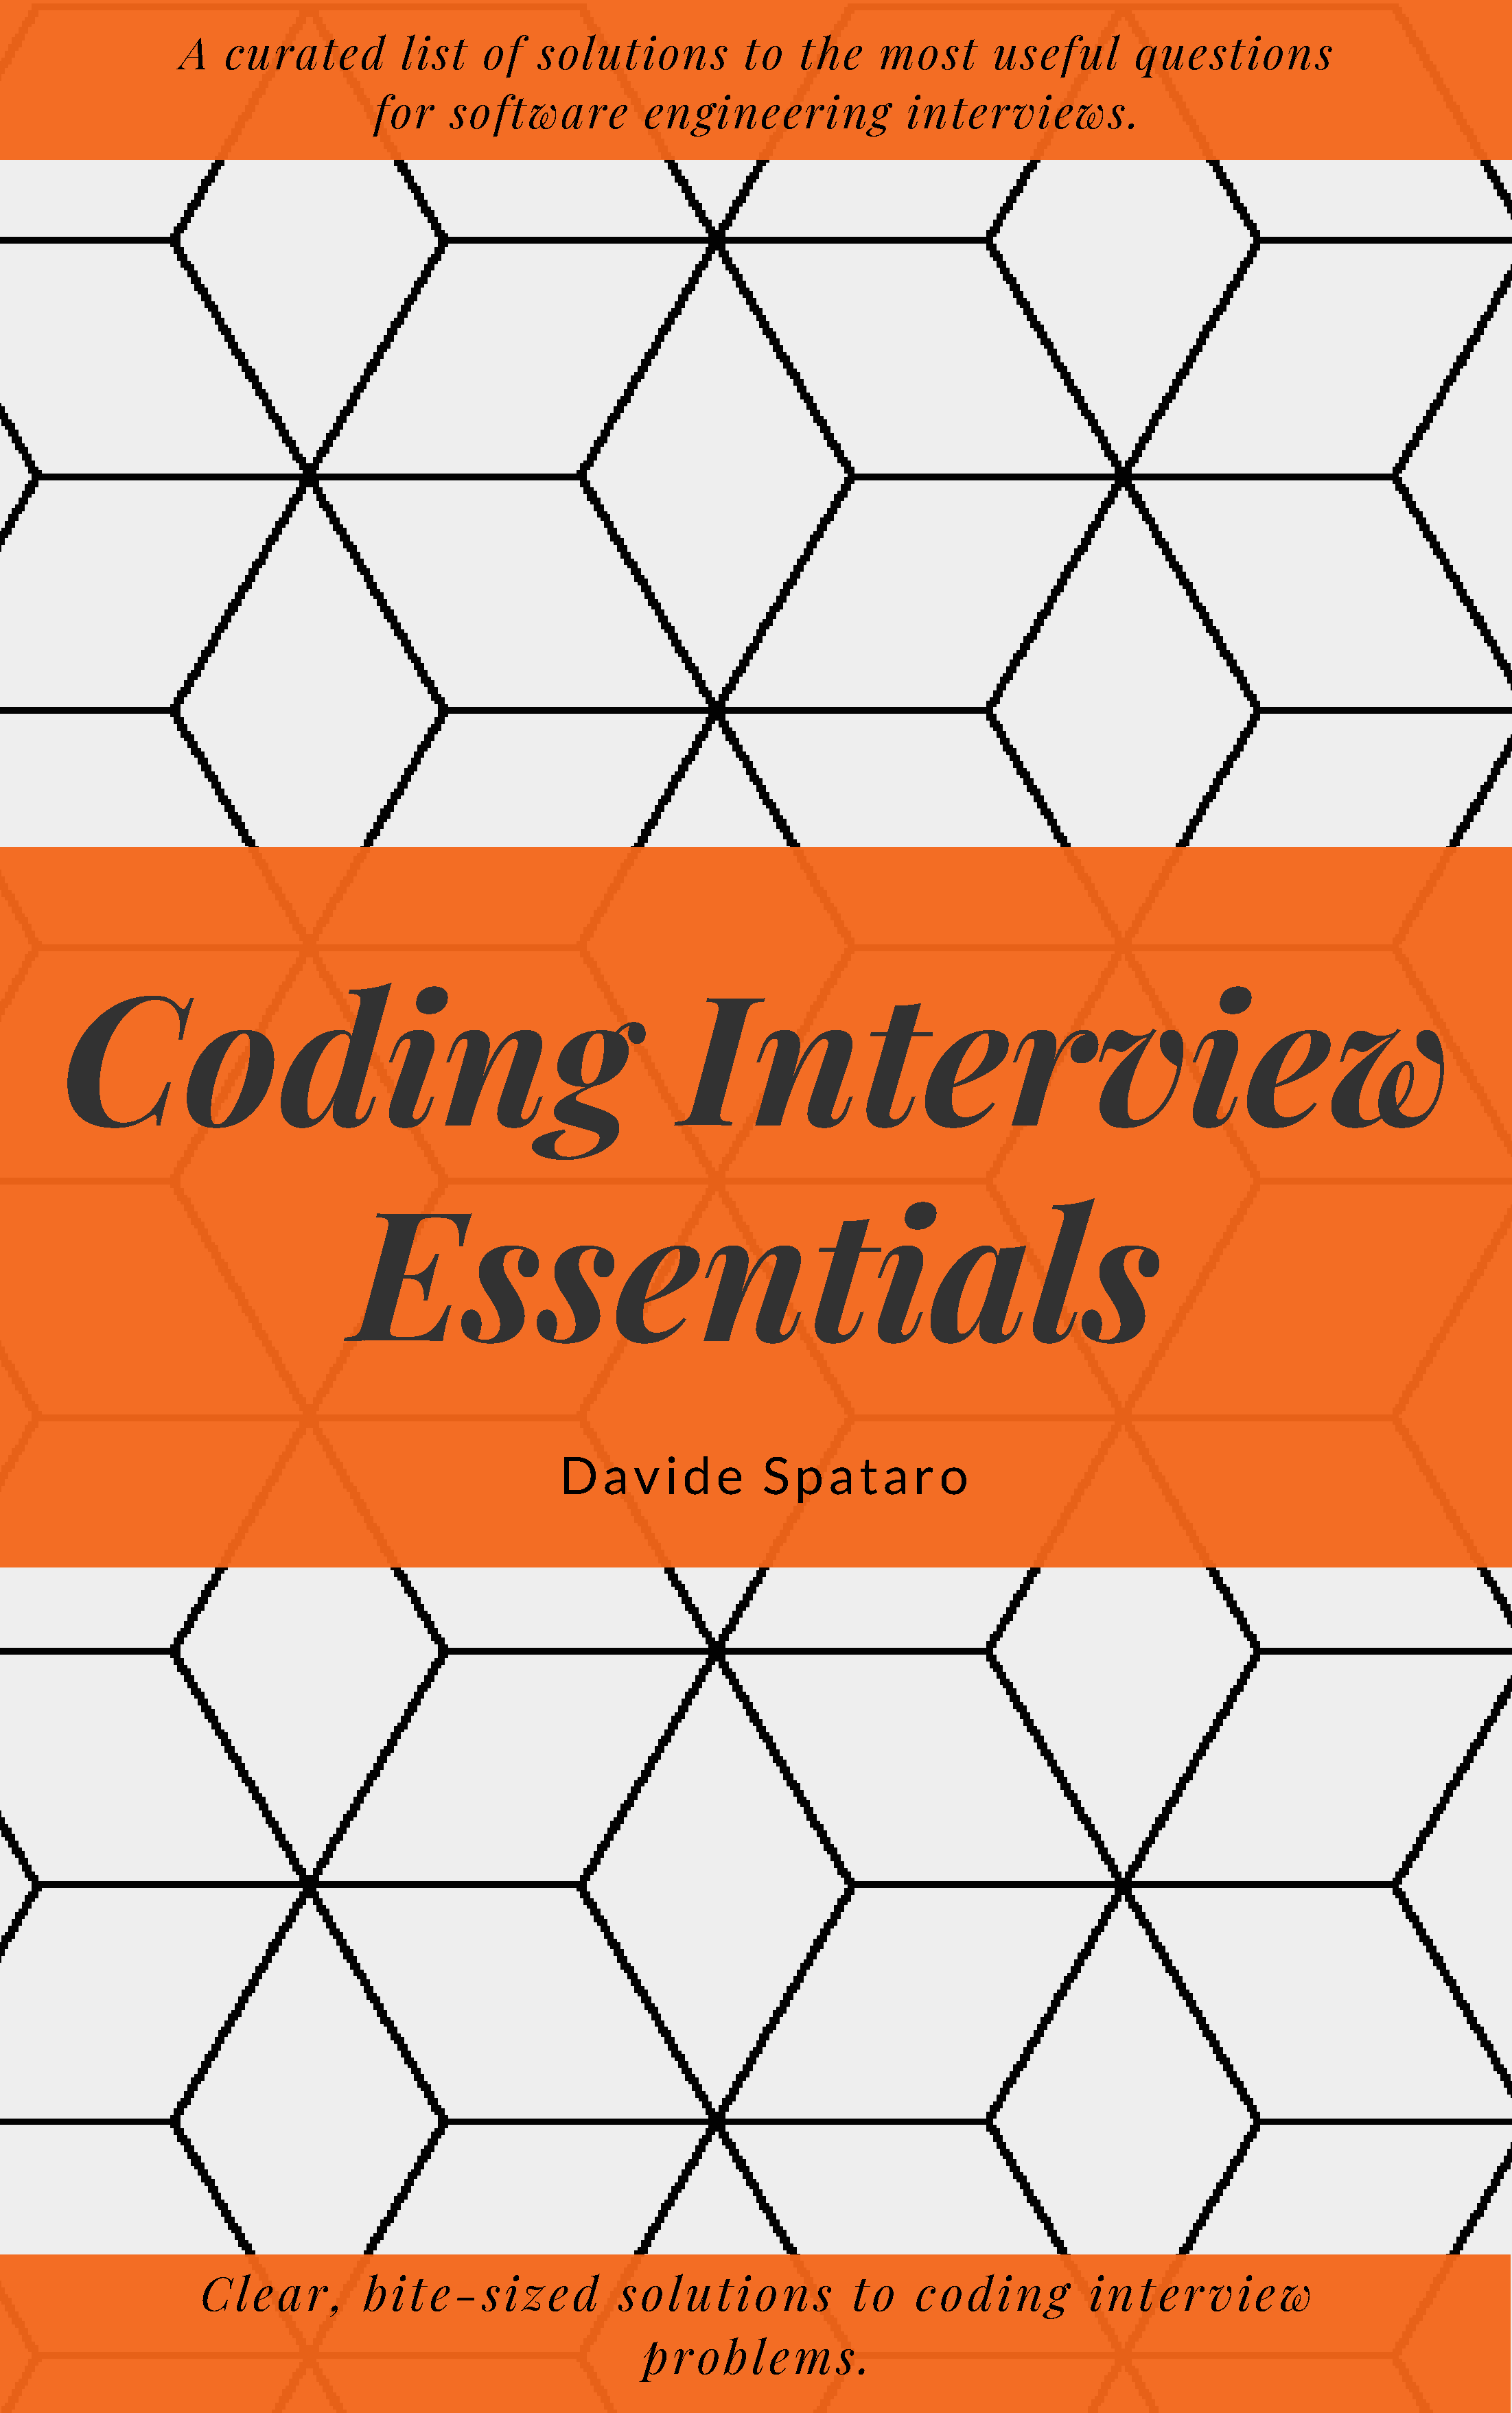
\includepdf[pages=1, fitpaper]{sources/front_cover_image.pdf}
%%\begingroup
%\thispagestyle{empty}
%\begin{tikzpicture}[remember picture,overlay]
%  \coordinate [below=12cm] (midpoint) at (current page.north);
%  \node at (current page.north west)
%  {\begin{tikzpicture}[remember picture,overlay]
%      \node[anchor=north west,inner sep=0pt] at (0,0) {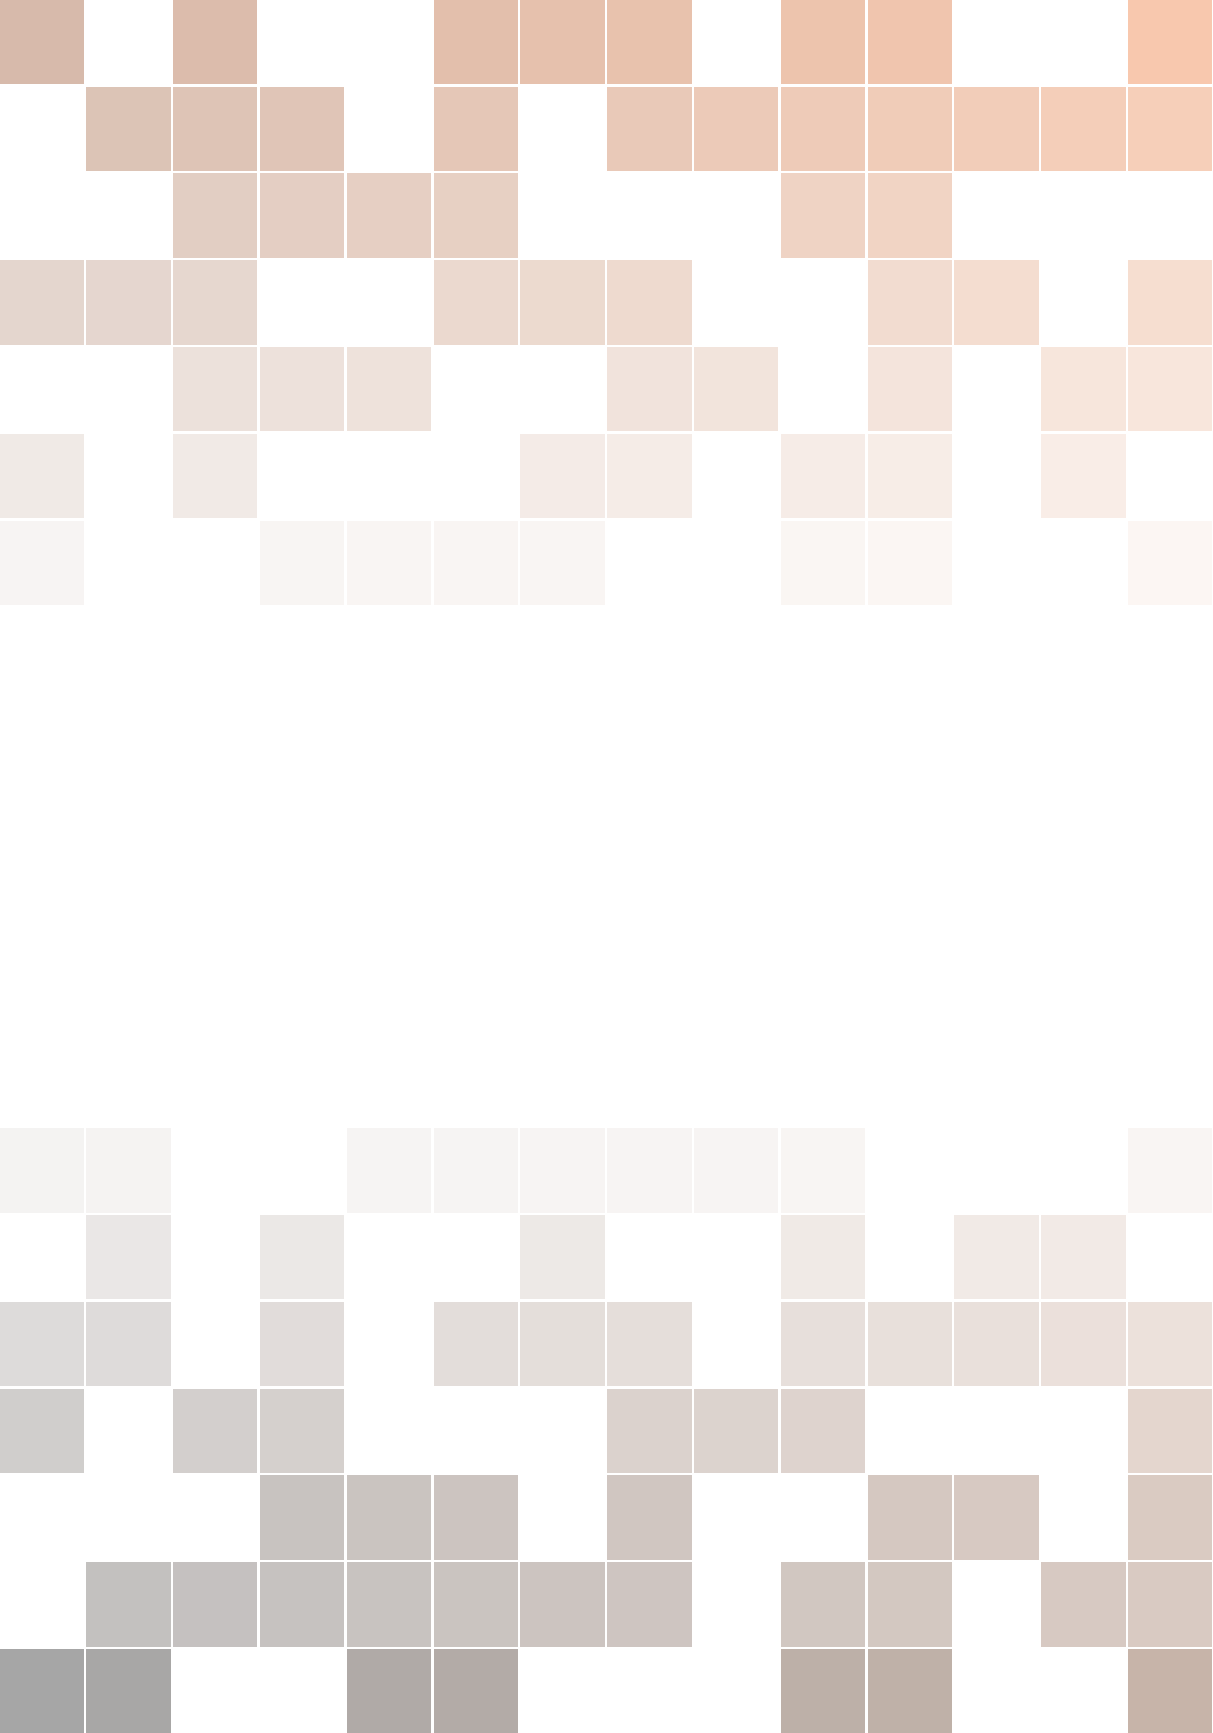
\includegraphics[width=\paperwidth]{images/background}}; % Background image
%\textsl{}
%      \draw[anchor=north] (midpoint) node [fill=ocre!30!white,fill opacity=0.6,text opacity=1,inner sep=1cm]{\Huge\centering\bfseries\sffamily\parbox[c][][t]{\paperwidth}{\centering Coding Interview Essentials\\[15pt] % Book title
%      {\Large - }\\[20pt] % Subtitle
%      {\huge Davide Spataro}}}; % Author name
%    \end{tikzpicture}};
%\end{tikzpicture}
%\vfill
%\endgroup


\includepdf[pages={2},fitpaper=true]{images/book_covers1.pdf}


\usechapterimagefalse % If you don't want to include a chapter image, use this to toggle images off - it can be enabled later with \usechapterimagetrue

%\chapterimage{images/header} % Table of contents heading image

\pagestyle{empty} % No headers

\tableofcontents % Print the table of contents itself

%\lstlistoflistings
%\listoffigures
%\listoftables

\cleardoublepage % Forces the first chapter to start on an odd page so it's on the right

%pagestyle{fancy} % Print headers again
%!TEX root = ../main.tex
%%%%%%%%%%%%%%%%%%%%%%%%%%%%%%%%%%
% Links:
%
% Difficulty:
% Companies: 
%%%%%%%%%%%%%%%%%%%%%%%%%%%%%%%%%%

\chapter{Best time to buy and sell stock}
\label{ch:buy_sell_stocks}
\section*{Introduction}
The problem discussed in this chapter is not particularly difficult as it is easily solvable in quadratic time using a brute-force algorithm. 
However, a more efficient solution is possible and, given that this is exactly the type of question for which interviewers expect fast and elegant solutions, it's worth taking the time to become familiar with the problem structure and the best approaches to solving it.  

\section{Problem statement}
\label{sec:buy_sell_stocks:statement1}
\begin{exercise}
You are given prices for a stock for a number $n$ of days. The prices are stored in an array $P$ of length $n$ where each cell $i$ of the array contains the price for the stock on the $i^{th}$ day. You are only permitted to perform \textbf{one} buy and \textbf{one} sell operations. What is the maximum profit you can achieve given the prices for the stock in $P$?

You have to perform the buy operation \textbf{before} the sell operation. You cannot buy the stock on the \nth{10} day and sell on the \nth{9}.

\begin{example}
	\hfill \\
	Given the array of prices for the stock is: $[7,1,5,3,6,4]$, the answer is $5$. You can buy on the \nth{2} day and sell on the \nth{5}.
\end{example}

\begin{example}
	\hfill \\
	Given the array of prices for the stock is: $[6,5,4,3,2,1]$, the answer is $0$. There is no way you can make a profit higher than $0$ i.e. not buying and not selling. 
\end{example}

\end{exercise}

\section{Clarification Questions}

\begin{QandA}
	\item \begin{questionitem} \begin{question} Can you perform the buy and sell operation on the same day?  \end{question}      
    \begin{answered}
		\textit{Yes, that is possible.}
	\end{answered} \end{questionitem}
\end{QandA}

\section{Discussion}
\label{buy_sell_stocks:sec:discussion}
A profit is achieved when a buy and sell transaction are performed with prices $p_b$ and $p_s$ respectively and $p_b \leq p_s$. In other words, our goal is to buy at a lower price than we sell. The maximum profit is obtained whenever the spread between those two prices is maximum i.e. $\max_{}{(p_s - p_b)}$

\subsection{Brute-force}
\label{buy_sell_stocks:sec:bruteforce}
The brute force approach is very straightforward as the only thing we need to do is apply the definition of maximum profit we discussed earlier. For all pairs of ordered index $i \leq j$ we can calculate $P_i - P_j$ and return the maximum among all those profit values. Listing \ref{list:buy_sell_stocks:bruteforce} shows an implementation of this approach. Note that a profit of $0$ is always possible by either not performing any transaction or simply performing the buy and sell on the same day. Thus $j = i+1$, because it is pointless to calculate the profit for the same day as we know already it will always be $0$. For this reason we also limit the buy operation to the day before ($i< n-1$) the last, because if we want to have any chance of making a profit we need to at least have one day left after the buy to perform the sell operation. 

\lstinputlisting[language=c++, caption={Brute force $O(n^2)$ solution to the problem of buying and selling stock.},label=list:buy_sell_stocks:bruteforce]{sources/buy_sell_stocks/buy_sell_stocks_solution1.cpp}

\subsection{Linear time solution}
\label{buy_sell_stocks:sec:linear}
The solution above can be improved if we look at the problem from slightly different angle. The idea is that we can process the array from the last day to the first and, for each of the days, calculate the \textbf{best} profit to be made by selling on any of the days already processed (which occurs later in time).

We keep a variable $b$ with the maximum price seen so far which is initially $-\infty$. The algorithm starts from day $n$ and for each day checks whether buying that day and selling at the price $b$ (the highest price seen so far) would improve the profit found thus far. This approach is correct because the maximum profit happens when the spread between sell and buy price is maximum.
The implementation of the idea above is shown in Listing \ref{list:buy_sell_stocks:linear}.

\lstinputlisting[language=c++, caption={Dynamic programming linear time, constant space solution to the problem of buying and selling stock.},label=list:buy_sell_stocks:linear]{sources/buy_sell_stocks/buy_sell_stocks_solution2.cpp}


%Multiple transaction variation
\section{Common Variations - Multiple Transactions}
\label{sec:buy_sell_stocks:multiple_transaction}

\subsection{Problem statement}
\begin{exercise}
	You are given an integer array $P$ where $P[i]$ contains the price of a given stock on the $i^{th}$ day.

	On each day, you may decide to buy and/or sell the stock. 
	You can only hold at most one share of the stock at any given time.
	However, you might engage in multiple transaction over the course of time i.e. you repeat the process of buying a share then sell it after a while (also the next day) multiple times.
	
	Write a function that given $P$ returns the maximum profit achievable.

	Notice that you may not engage in multiple transactions at the same time i.e., you must sell the stock before you buy it again.
	\begin{example}
	\label{ex:buy_sell_stocks_2:exmaple1}
		\hfill \\
		Given the array of prices for the stock is: $[7,1,5,3,6,4]$, the answer is $7$. 
		You can buy on the \nth{2} day and sell on the \nth{3} and then engage on a second transaction where you buy on the \nth{4} day and sell on the \nth{5}.
	\end{example}

\end{exercise}


\section{Discussion}
\label{buy_sell_stocks_2:sec:discussion}
This might seems like an harder problem at first than the version presented in Section \ref{sec:buy_sell_stocks:statement1} but in reality as we will see in Section \ref{buy_sell_stocks_2:sec:linear} its solution is actually easier.

\section{Brute force solution}
\label{buy_sell_stocks_2:sec:bruteforce}
As usual we start our discussion by quickly presenting the brute force solution. In this case this means trying all possible sets of transactions (a valid pair of buy and sell operation not overlapping with any other transaction). We can try all possible sets by using recursion cleverly. However this approach will not take us far because the number of possible sets of transaction grows exponentially.
We are showing this approach in Listing \ref{list:buy_sell_stocks_2:bruteforce}  only because we think its implementation can be somehow instructive.

\lstinputlisting[language=c++, caption={Bruteforce exponential solution to the problem of buying and selling stock with no limits on the number of transactions.},label=list:buy_sell_stocks_2:bruteforce]{sources/buy_sell_stocks/buy_sell_stocks_2/buy_sell_stocks_2_solution1.cpp}

\section{Linear time solution}
\label{buy_sell_stocks_2:sec:linear}


The idea is simple and it is clearer once we look at prices plotted on a graph. As you can see in Figure \ref{}, the data is made of peaks and valleys (unless the data is fully increasing or decreasing). Those are the point of interests because if we buy at valleys and sell at peaks we are able to obtains the maximum profit. 
One can simply loop thought the array and identify those peaks and valleys and calculate the total profit as the sum of the profits along those point of interests. 
For instance w.r.t. the example \ref{ex:buy_sell_stocks_2:exmaple1} there are two pairs  valley-peak happening at days $2$ and $3$ and days $4$ and $5$, respectively. 
But, what is a valley and/or a peak exactly?
A day $i$ is a valley if $P_i < P_{i-1}$ and $P_i > P_{i+1}$
while is a peak if $P_i > P_{i-1}$ and $P_i < P_{i+1}$.
So all it is needed is to identify those pairs of valleys and peaks and we are done. 

But do we really need to find peaks and valleys? The answer is not as all it is necessary is to make sure we cash at \textbf{all} opportunities we have i.e. in all those cases where we can buy at a lower price we sell. Thus we can process days two at the time and, since there is no limit on the number of transactions, simply buy and sell whenever the spread between buy and sell price is convenient. 

The idea above can be implemented as shown in Listing \ref{list:buy_sell_stocks_2:linear}. 


\lstinputlisting[language=c++, caption={$O(n)$ time and $O(1)$ space solution to the problem of buying and selling stock with no limits on the number of transactions.},label=list:buy_sell_stocks_2:linear]{sources/buy_sell_stocks/buy_sell_stocks_2/buy_sell_stocks_2_solution2.cpp}


%%%%%%%%%%%%%%%%%%%%%%%%%%%%%%%%%%%%%%%%%%%%
%               Appendices
%%%%%%%%%%%%%%%%%%%%%%%%%%%%%%%%%%%%%%%%%%%%

\chapter{Appendices}
%% @Author: Davide Spataro
% @Date:   2020-10-25 
% @Last Modified by:   Davide Spataro
% https://www.topcoder.com/community/competitive-programming/tutorials/dynamic-programming-from-novice-to-advanced/
% file:///home/knotman/Downloads/DYNAMIC_PROGRAMMING_-_ITS_PRINCIPLES_APPLICATIONS_.pdf
% http://smo.sogang.ac.kr/doc/bellman.pdf 
\section*{Dynamic Programming}
\label{sect:appendix:DP}

Dynamic programming (DP) is a popular technique for solving a certain class of
optimization problems efficiently and is accredited to the American Scientist
Richard Bellman\cite{bellman1954}. He conied the term DP in the context of
solving problems involving a serie of best decision one after the other. 
The word \textit{programming} can be a bit deceiving for
computer scientist of programmers in general but it has really little to do with
computer programming and it is infact intended as a set of rules to 
follow to solve a certain problem and it is refeered specifically to the
solution to find an optimal military schedule for logistics (and has more or
less the same meaning as linear programming or linear optimization).  These rules can of course be coded and
executed by a computer but can be easily followed on paper for instance. 
Dynamic programming is better thought as an optimization approach rather than an
method or framework where a complex optimization problem is transformed into a sequence of
smaller (and simpler) problems. The very essence of DP is its multi-stage
optimization procedure. DP does not provide directly with the
instruction on how to solve a particular problem, but instead provides a general
framework that requires creativity and non trivial effort/insights so that a
problem formulation can be adapted and casted within the DP framework bounds.
This is possibly the reason why DP is considered a rather hard topic and it is
particularly feared during interviews. 

This chapter is not intended to be a full treatement of DP, and we will
introduce and describe it to the level that is necessary to understand and
better tackle DP interview problems. For a more comprenshive material on DP
please refer to \cite{bellman1954, cormen2009}.

The gist of the DP approach is that we aim at breaking down a problem into
simpler sub-problems recursively. If it is possible to do so, then the problem
at hand is said to have the \textbf{optimal substructure} property i.e. it can
be solved by using optimal solution to subproblems. But having the optimal
substructure property alone is not enough to prefer a DP approach to another
when trying to solve the same problem. This is because DP really shines when a
problem also exposes the \textbf{overlapping subproblems} property i.e. when the
subproblems are reused several times. A classic example if the
Fibonacci Sequence. In order to calculate $F(n)$ we need to solve two subproblems:
$F(n-1)$ and $F(n-2)$ and adding them up. But for solving $F(n-1)$ we need to
solve $F(n-2)$ \textbf{again}. The value for the subproblem $F(n-2)$ is thus
reused and this makes the Fibonacci problem exposed the optimal substructure
property. 
Dynamic programming takes care of this fact by making sure of solving each
subproblem only once. Usually this can be achieved into two ways:
\begin{description}
    \item [Top-down] This is usually the easiest of the two, by being a direct
    derivation from the recursive formulation of the problem. If the problem can
    be formulated recursively in terms of solution then solution to subproblems
    can be \textit{memoized}\footnote{From the latin word \textit{memorandum}
    which means to be remembered. It is basically a way of remembering the
    result of a function for a certain set of inputs call by storing it in a
    cache.} in a cache. 
    When a subproblem is reused then the
    (potentially expensive) recursive call is avoided and the cached result is
    returned instead. 
    \item [Bottom-up] We can try to reformulate the problem by twisting and
    massaging  the  recursive formulation so that the subproblems are solved
    first (thus effectively removing the recursion) and build the solution to
    the bigger problem from the bottom. This is usually done by working in a
    sort of tabular form where entries of the table for larger problems are
    filled by using  entries for solution to smaller problems that we have
    already solved. For instance, when solving the problem of finding the
    $10^{th}$ Fibonacci number $F(10)$, we can start from the known values for
    $F(0)$ and $F(1)$ and working our way up to $F(2)$  by using $F(1)$ and
    $F(2)$. Once F(2) is ready we can move up to F(3), and so on when we have
    the values for $F(8)$ and $F(9)$ we proceed with calculating $F(10)$.
\end{description}

DP has found application in many field of science such as Control theory,
Bioinformatics AI and operations research. There are a number of problems in
computer science that can be solved by using DP such as the 
\begin{itemize}
    \item Longest Common (or increasing) Subsequence
    \item Weighted Interval Scheduling
    \item Chain Matrix Multiplication
    \item Subset sub
    \item String edit distance
    \item Coin change
    \item 0/1 knapsack problem
    \item Graph shortest path
\end{itemize}

In the next section we will shortly review a number of DP problem focusing on
the key ideas that allow a problem to be approached and solved  using DP.

\subsection*{Fibonacci Sequence}
Computing the $n^{th}$ number of the Fibonacci sequence is probably one of the
most common introductionary example of DP. The Fibonacci sequence recursive
formulation is ready to be solved using a top-down DP approach. Listing
\ref{list:app:dp:canonical} shows a C++ function that calculated the $n^{th}$ Fibonacci
number.
\lstinputlisting[language=c++, caption={Canonical recursive C++ implementation of a function returning the $n^{th}$ Fibonacci number.},label=list:app:dp:canonical]{/home/dspataro/git/algorithm_articles/sources/appendices/fibonacci_canonical.cpp}
Notice that for instance when $F(6)$ a call tree is produced where the same call
is repeated more than once as shown in the list below. $F(2)$ has been
calculated $5$ times!
\begin{itemize}
    \item $F(6) = F(5)+F(4)$
    \item $F(6) = (F(4)+F(3)) + (F(3)+F(2))$
    \item $F(6) = ((F(3)+F(2))+(F(2)+F(1))) + ((F(2)+F(1))+(F(1)+F(0)))$
    \item $F(6) = (((F(2)+F(1))+(F(1)+F(0)))+((F(1)+F(0))+F(1))) + (((F(1)+F(0))+F(1))+(F(1)+F(0)))$
    \item $F(6) = ((((F(1)+F(0))+F(1))+(F(1)+F(0)))+((F(1)+F(0))+F(1))) + (((F(1)+F(0))+F(1))+(F(1)+F(0)))$
\end{itemize}

Listing \ref{list:app:dp:fib} can be improved dramatically if we memoize the function calls
that have been already calculated. This way no duplicate work is done. W.r.t the
previous example, from the second time the value of $F(2)$ is needed, no
additional work is done, as the value in the cache is returned.
\lstinputlisting[language=c++, caption={Canonical recursive top-down Dynamic Programming C++ implementation of a function returning the $n^{th}$ Fibonacci number.},label=list:app:dp:fib]{/home/dspataro/git/algorithm_articles/sources/appendices/fibonacci_dp_top_down.cpp}

%\section{Prefix sum}
\label{sect:appendix:prefix_sum}
In computer science, the prefix sum, cumulative sum, inclusive scan, or simply scan of a sequence of numbers x0, x1, x2, ... is a second sequence of numbers y0, y1, y2, ..., the sums of prefixes (running totals) of the input sequence:
%% @Author: Davide Spataro
% @Date:   2020-03-30 17:18:14
% @Last Modified by:   Davide Spataro
% @Last Modified time: 2020-03-30 17:28:08
\section{Binary Search}
\label{sect:appendix:binary_search}
\lipsum{1}
\lstinputlisting[language=c++, caption={},label=list:listings:hash_pair]{test/common/hash_pair.h}

\section*{Latencies Reference}
\FloatBarrier
\begin{table}[]
    \centering
    \resizebox{\textwidth}{!}{%
    \begin{tabular}{lllll}
    \hline
    \rowcolor[HTML]{C0C0C0} 
    \multicolumn{1}{c}{\cellcolor[HTML]{C0C0C0}\textbf{Operation}}     & \multicolumn{3}{c}{\cellcolor[HTML]{C0C0C0}\textbf{Latency}}               & \multicolumn{1}{c}{\cellcolor[HTML]{C0C0C0}\textbf{Notes}} \\ \hline
    \rowcolor[HTML]{C0C0C0} 
                                                                       & \textit{\textbf{nano}} & \textit{\textbf{micro}} & \textit{\textbf{milli}} &                                                            \\
    \textit{L1 cache reference}                                        & 0.5                    & 0.000500000             & 0.000000500             & 14 \textbackslash{}times L1 cache                          \\
    \textit{Branch mispredict}                                         & 5                      & 0.005000000             & 0.000005000             &                                                            \\
    \textit{L2 cache reference}                                        & 7                      & 0.007000000             & 0.000007000             &                                                            \\
    \textit{Mutex lock/unlock}                                         & 25                     & 0.025000000             & 0.000025000             &                                                            \\
    \textit{Main Memory Reference}                                     & 100                    & 0.100000000             & 0.000100000             & 20 times L2 cache. 200x L1                                 \\
    \textit{Compress 1K bytes with Zippy}                              & 3000                   & 3.000000000             & 0.003000000             &                                                            \\
    \textit{Send 1K bytes over 1 Gbps network}                         & 10000                  & 10.000000000            & 0.010000000             &                                                            \\
    \textit{Read 4K randomly from SSD*}                                & 150000                 & 150.000000000           & 0.150000000             & $\sim$1GB/sec SSD                                          \\
    \textit{Round trip within same datacenter}                         & 500000                 & 500.000000000           & 0.500000000             &                                                            \\
    \textit{Read 1 MB sequentially from SSD*}                          & 1000000                & 1000.000000000          & 1.000000000             & $\sim$1GB/sec SSD, 4X memory                               \\
    \textit{Disk seek}                                                 & 10000000               & 10000.000000000         & 10.000000000            & 20x datacenter roundtrip                                   \\
    \textit{Read 1 MB sequentially from disk}                          & 20000000               & 20000.000000000         & 20.000000000            & 80x memory, 20X SSD                                        \\
    \textit{Send packet CA-\textgreater{}Netherlands-\textgreater{}CA} & 150000000              & 150000.000000000        & 150.000000000           &                                                           
    \end{tabular}%
    }
    \caption{Latency Comparison Numbers ($\sim$2012). Credit to \url{https://gist.github.com/jboner/2841832}}
    \label{tab:refernce_latencies}
\end{table}
\FloatBarrier


\begin{figure}
	\centering
	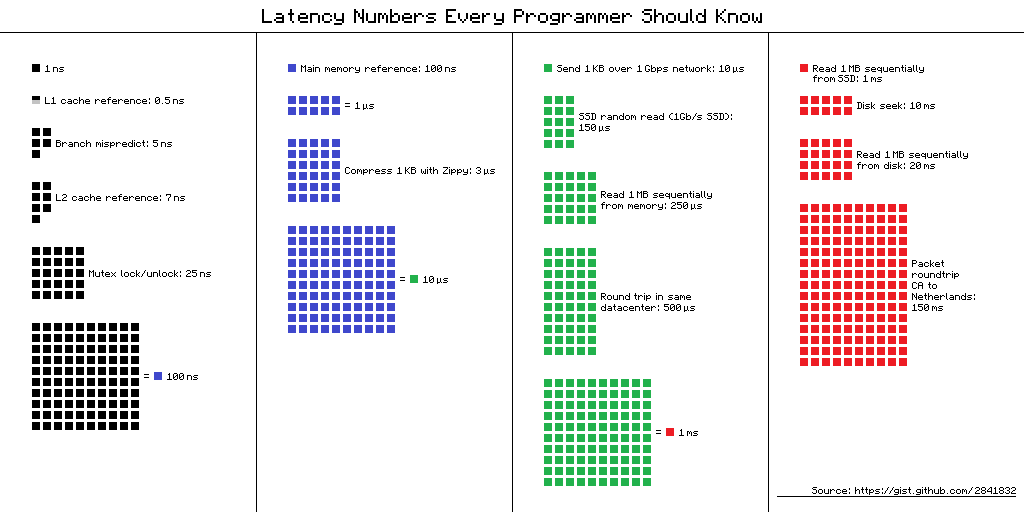
\includegraphics[width=\textwidth]{sources/appendices/images/latencies-refernece.png}
	\caption[]{Humanized visualization of the data in Table 
    \ref{tab:refernce_latencies}}.
	\label{fig:refernce_latencies}
\end{figure}

\FloatBarrier

\vspace{-2cm}
\section*{Data structures Asymptotic complexity cheatsheet}
% Please add the following required packages to your document preamble:
% \usepackage{booktabs}
% \usepackage{multirow}
% \usepackage{graphicx}
% \usepackage[table,xcdraw]{xcolor}
% If you use beamer only pass "xcolor=table" option, i.e. \documentclass[xcolor=table]{beamer}
\begin{table}[!htbp]
    \centering
    \resizebox{\textwidth}{!}{%
    \begin{tabular}{@{}lccccccccc@{}}
    \toprule
                                              & \multicolumn{8}{l}{\textbf{Time Complexities}}                                                                                                                                                                                                                                                                                                                                                  & \multicolumn{1}{l}{\textbf{Space Complexity}}             \\ \cmidrule(l){2-10} 
                                              & \multicolumn{1}{l}{\textbf{Average case}}    & \multicolumn{7}{l}{\textbf{Worst case}}                                                                                                                                                                                                                                                                                                          & \multicolumn{1}{l}{}                                      \\
    \multirow{-3}{*}{\textbf{Data Structure}} & \multicolumn{1}{l}{\textit{\textbf{Access}}} & \multicolumn{1}{l}{\textit{\textbf{Search}}} & \multicolumn{1}{l}{\textit{\textbf{Insertion}}} & \multicolumn{1}{l}{\textit{\textbf{Deletion}}} & \multicolumn{1}{l}{\textit{\textbf{Access}}} & \multicolumn{1}{l}{\textit{\textbf{Search}}} & \multicolumn{1}{l}{\textit{\textbf{Insertion}}} & \multicolumn{1}{l}{\textit{\textbf{Deletion}}} & \multicolumn{1}{l}{\multirow{-2}{*}{\textbf{Worst case}}} \\ \cmidrule(r){1-1}
    Array                                     & \cellcolor[HTML]{009901}$O(1)$               & \cellcolor[HTML]{FFC702}$O(n)$               & \cellcolor[HTML]{FFC702}$O(n)$                  & \cellcolor[HTML]{FFC702}$O(n)$                 & \cellcolor[HTML]{009901}$O(1)$               & \cellcolor[HTML]{FFC702}$O(n)$               & \cellcolor[HTML]{FFC702}$O(n)$                  & \cellcolor[HTML]{FFC702}$O(n)$                 & \cellcolor[HTML]{FFC702}$O(n)$                            \\
    Stack                                     & \cellcolor[HTML]{009901}$O(1)$               & \cellcolor[HTML]{656565}N.A.                 & \cellcolor[HTML]{009901}$O(1)$                  & \cellcolor[HTML]{009901}$O(1)$                 & \cellcolor[HTML]{009901}$O(1)$               & \cellcolor[HTML]{656565}N.A.                 & \cellcolor[HTML]{009901}$O(1)$                  & \cellcolor[HTML]{009901}$O(1)$                 & \cellcolor[HTML]{FFC702}$O(n)$                            \\
    Queue                                     & \cellcolor[HTML]{009901}$O(1)$               & \cellcolor[HTML]{656565}N.A.                 & \cellcolor[HTML]{009901}$O(1)$                  & \cellcolor[HTML]{009901}$O(1)$                 & \cellcolor[HTML]{009901}$O(1)$               & \cellcolor[HTML]{656565}N.A.                 & \cellcolor[HTML]{009901}$O(1)$                  & \cellcolor[HTML]{009901}$O(1)$                 & \cellcolor[HTML]{FFC702}$O(n)$                            \\
    Singly Linked List                        & \cellcolor[HTML]{FFC702}$O(n)$               & \cellcolor[HTML]{FFC702}$O(n)$               & \cellcolor[HTML]{009901}$O(1)$                  & \cellcolor[HTML]{FFC702}$O(n)$                 & \cellcolor[HTML]{FFC702}$O(n)$               & \cellcolor[HTML]{FFC702}$O(n)$               & \cellcolor[HTML]{009901}$O(1)$                  & \cellcolor[HTML]{FFC702}$O(n)$                 & \cellcolor[HTML]{FFC702}$O(n)$                            \\
    Doubly Linked List                        & \cellcolor[HTML]{FFC702}$O(n)$               & \cellcolor[HTML]{FFC702}$O(n)$               & \cellcolor[HTML]{009901}$O(1)$                  & \cellcolor[HTML]{009901}$O(1)$                 & \cellcolor[HTML]{FFC702}$O(n)$               & \cellcolor[HTML]{FFC702}$O(n)$               & \cellcolor[HTML]{009901}$O(1)$                  & \cellcolor[HTML]{009901}$O(1)$                 & \cellcolor[HTML]{FFC702}$O(n)$                            \\
    Hash Table                                & \cellcolor[HTML]{009901}$O(1)$               & \cellcolor[HTML]{009901}$O(1)$               & \cellcolor[HTML]{009901}$O(1)$                  & \cellcolor[HTML]{009901}$O(1)$                 & \cellcolor[HTML]{FFC702}$O(n)$               & \cellcolor[HTML]{FFC702}$O(n)$               & \cellcolor[HTML]{FFC702}$O(n)$                  & \cellcolor[HTML]{FFC702}$O(n)$                 & \cellcolor[HTML]{FFC702}$O(n)$                            \\
    Binary Search Tree                        & \cellcolor[HTML]{32CB00}$O(log_2(n))$        & \cellcolor[HTML]{32CB00}$O(log_2(n))$        & \cellcolor[HTML]{32CB00}$O(log_2(n))$           & \cellcolor[HTML]{32CB00}$O(log_2(n))$          & \cellcolor[HTML]{FFC702}$O(n)$               & \cellcolor[HTML]{FFC702}$O(n)$               & \cellcolor[HTML]{FFC702}$O(n)$                  & \cellcolor[HTML]{FFC702}$O(n)$                 & \cellcolor[HTML]{FFC702}$O(n)$                            \\
    Red-Black Tree                            & \cellcolor[HTML]{32CB00}$O(log_2(n))$        & \cellcolor[HTML]{32CB00}$O(log_2(n))$        & \cellcolor[HTML]{32CB00}$O(log_2(n))$           & \cellcolor[HTML]{32CB00}$O(log_2(n))$          & \cellcolor[HTML]{32CB00}$O(log_2(n))$        & \cellcolor[HTML]{32CB00}$O(log_2(n))$        & \cellcolor[HTML]{32CB00}$O(log_2(n))$           & \cellcolor[HTML]{32CB00}$O(log_2(n))$          & \cellcolor[HTML]{FFC702}$O(n)$                            \\
    Heap                                      & \cellcolor[HTML]{009901}$O(1)$               & \cellcolor[HTML]{656565}N.A.                 & \cellcolor[HTML]{32CB00}$O(log_2(n))$           & \cellcolor[HTML]{32CB00}$O(log_2(n))$          & \cellcolor[HTML]{009901}$O(1)$               & \cellcolor[HTML]{656565}N.A.                 & \cellcolor[HTML]{32CB00}$O(log_2(n))$           & \cellcolor[HTML]{32CB00}$O(log_2(n))$          & \cellcolor[HTML]{FFC702}$O(n)$                            \\ \bottomrule
    \end{tabular}%
    }
    \caption{Asymptotic complexities for a number of data strucutes. For time, both the average and case is reported, while for space only the worst. $O(1) < O(log_2(n)) < O(log_2(n)) < O(n) < O(nlog_2(n) < O(n^2) < O(n^3) \ldots < O(2^n) < O(n!) < O(n^n)$  }
    \label{appendix:ds_complexities}
\end{table}


\begin{figure}
    \centering
\begin{tikzpicture}
    \begin{axis}[
      grid = major,
      clip = true,
      ticks = none,
      width=0.9\textwidth,
      height=0.7\textwidth,
      every axis plot/.append style={very thick},
      axis line style = ultra thick,
      clip mode=individual,
      restrict y to domain=0:40,
      restrict x to domain=0:20,
      axis x line = left,
      axis y line = left,
      domain = 0.00:10,
      xmin = 0,
      xmax = 11,
      ymin = 0,
      ymax = 42,
      xlabel = n,
      ylabel = no. of operations,
      xlabel style = {at={(axis description cs:0.5,-0.1)},anchor=south},
      ylabel style = {at={(axis description cs:-0.08,0.5)},anchor=north},
      label style = {font=\LARGE\bf},
    ]
  \addplot [
      samples=100, 
      color=red,
  ]
  {x^2}node[above,pos=1,style={font=\Large}]{$\mathcal{O}(n^2)$};
  \addplot [
      samples=100, 
      color=blue,
  ]
  {x}node[above,pos=1,style={font=\Large}]{$\mathcal{O}(n)$};
  \addplot [
      samples=100, 
      color=orange,
  ]
  {log2 x}node[above,pos=1,style={font=\Large}]{$\mathcal{O}(\log{}n)$};
  \addplot [
      samples=100, 
      color=black,
  ]
  {x*(log2 x)}node[above,pos=1,style={font=\Large}]{$\mathcal{O}(n\log{}n)$};
  \addplot [
      samples=100, 
      color=magenta,
  ]
  {1}node[above,pos=1,style={font=\Large}]{$\mathcal{O}(1)$};
  \addplot [
      samples=100, 
      color=cyan,
  ]
  {x^(2.2)}node[above,pos=1,style={font=\Large}]{$\mathcal{O}(n^3)$};
  

  \addplot [
    samples=100,
    color=green, 
  ] gnuplot{gamma(x+3)} node[above,pos=1,style={font=\Large}]{$\mathcal{O}(n!)$};

  \addplot [
    samples=100, 
    color=yellow,
]
{2.5*2^x}node[above,pos=1,style={font=\Large}]{$\mathcal{O}(2^x)$};
  
  \end{axis}
  \end{tikzpicture}

  \caption[]{Graph showing the relative growth rates of common function used to describe algorithms.}
  \label{fig:ds_complexities:graph}
\end{figure}
%%%%%%%%%%%%%%%%%%%%%%%%%%%%%%%%%%%%%%%%%%%%
%               BIBLIOGRAPHY
%%%%%%%%%%%%%%%%%%%%%%%%%%%%%%%%%%%%%%%%%%%%

%
%from documentation
%\newacronym[⟨key-val list⟩]{⟨label ⟩}{⟨abbrv ⟩}{⟨long⟩}
%above is short version of this
% \newglossaryentry{⟨label ⟩}{type=\acronymtype,
% name={⟨abbrv ⟩},
% description={⟨long⟩},
% text={⟨abbrv ⟩},
% first={⟨long⟩ (⟨abbrv ⟩)},
% plural={⟨abbrv ⟩\glspluralsuffix},
% firstplural={⟨long⟩\glspluralsuffix\space (⟨abbrv ⟩\glspluralsuffix)},
% ⟨key-val list⟩}

\newacronym{cd}{CD}{compact disk}
\newacronym{utc}{UTC}{Coordinated Universal Time}
%\newacronym{adt}{ADT}{Atlantic Daylight Time}
%\newacronym{est}{EST}{Eastern Standard Time}
 
% Use the acronyms
\gls{utc} is 3 hours behind \gls{adt} and 10 hours ahead of \gls{est}.



%\addcontentsline{toc}{chapter}{\textcolor{ocre}{Glossary}}
%\printglossaries


%Print the glossary

\addcontentsline{toc}{chapter}{\textcolor{ocre}{Bibliography}}
%\chapter*{Bibliography}
%Print the glossary
\printbibliography	
	
%%%%%%%%%%%%%%%%%%%%%%%%%%%%%%%%%%%%%%%%%%%%
%               INDEX
%%%%%%%%%%%%%%%%%%%%%%%%%%%%%%%%%%%%%%%%%%%%	
	\cleardoublepage
	\phantomsection
	\setlength{\columnsep}{0.75cm}
	\addcontentsline{toc}{chapter}{\textcolor{ocre}{Index}}
	\printindex


	%\backmatter

\end{document}
